\documentclass{article}

% Language setting
% Replace `english' with e.g. `spanish' to change the document language
\usepackage[portuguese]{babel}

% Set page size and margins
% Replace `letterpaper' with `a4paper' for UK/EU standard size
\usepackage[letterpaper,top=2cm,bottom=2cm,left=3cm,right=3cm,marginparwidth=1.75cm]{geometry}

% Useful packages
\usepackage{amsmath}
\usepackage{graphicx}
\usepackage[colorlinks=true, allcolors=blue]{hyperref}

\title{MAP2212 - Exercício de Programação 1}
\author{Lucas Panfilo Donaire - 12556552}

\begin{document}
\maketitle

\begin{abstract}
Usando um Método de Monte Carlo para estimar $\pi$ computacionalmente através de geração de pontos aleatórios no quadrado unitário.
\end{abstract}

\section{Introdução}
\subsection{Métodos de Monte Carlo}

A \href{https://pt.wikipedia.org/wiki/Lei_dos_grandes_n%C3%BAmeros
} {Lei dos grandes números}, ideia fundamental da teoria da probabilidade, foi primeiramente formulada por Jacob Bernoulli: "Para um grande número de experiências, tendo cada uma um resultado aleatório, a frequência relativa de cada um desses resultados tende a estabilizar, convergindo para um certo número que constitui a probabilidade desse resultado".

Disso concluimos que, quando repetimos um experimento, na medida que o número de tentativas aumenta, a média aritmética dos resultados do experimento tende a se aproximar de seu valor esperado. 

Assim surgem os chamados \href{https://pt.wikipedia.org/wiki/M%C3%A9todo_de_Monte_Carlo
} {Métodos de Monte Carlo}, métodos que usam amostragens aleatórias massivas para obter resultados numéricos sobre alguma distribuição. Tais métodos são úteis para obter aproximações numéricas.

\subsection{Simulação do valor de $\pi$}

Como estimar o valor de $\pi$ computacionalmente? Bom, se nos foi dado que a área de um círculo de raio 1 é $\pi$, então só precisamos usar um Método de Monte Carlo: 

\begin{itemize}
    \item Simulamos $n$ pontos aleatoriamente no quadrado unitário [-1,1]$\times$[-1,1], o qual tem área total 4 e contém nosso círculo de raio 1 e centro na origem.
    \item Contamos a quantidade $P$ de quantos pontos estão dentro do circúlo unitário
    \item Pela Lei dos grandes números, a proporção $P/n$ deve se aproximar de $\pi$/4 conforme n cresce.
\end{itemize}



\section{Número de simulações}

\subsection{Erro e confiança}

Já sabemos o algorítmo para aproximar pi, mas se queremos uma aproximação suficientemente boa, temos que ajustar o número de pontos simulados para nos dar certa confiabilidade. Vamos procurar um erro menor ou igual a 0,005\% com confiança de 0,95\% 

\newpage
\subsection{Em busca do tamanho de amostra ideal}

Enunciaremos alguns teoremas e resultados de probabilidade e estatística para estimar n a seguir. 

\subsubsection{Teorema central do limite}

Sejam $X_1, X_2, \ldots, X_n$ uma amostra aleatória simples da população $X$, tal que $\text{E}[X_i] = \mu$ e $\text{Var}[X_i] = \sigma^2 < \infty$. Seja
\[X_m = \frac{X_1 + X_2 + \cdots + X_n}{n}
      = \frac{1}{n}\sum_{i}^{n} X_i\]
a média amostral da amostra. Então, conforme $n$ tende a infinito, a variável aleatória $X_m$ converge para uma distribuição normal $\mathcal{N}(\mu, \sigma^2/n)$.

\subsubsection{Tamanho de amostras de distribuições normais}

Suponha que estejamos estimando a média $\mu$ populacional para tanto usaremos a média amostral, $X_m$, baseada numa amostra de tamanho n. Suponha
que se queira determinar o valor de n de modo que \\
\[P(|X_m - \mu| \leq \varepsilon) \geq \gamma \] 
com $0 < \gamma < 1$, e $\varepsilon$ é o erro amostral máximo que podemos suportar, ambos valores fixados.
Sabemos que $X_m$ tem distribuição $\mathcal{N}(\mu, \sigma^2/n)$. Então: \\
\[ P(-\varepsilon \leq X_m - \mu \leq \varepsilon) = P(\frac{-\varepsilon \sqrt{n}}{\sigma} \leq Z \leq \frac{\varepsilon \sqrt{n}}{\sigma} ) \approx \gamma , \]
com $Z = \frac{(X_m–\mu)\sqrt{n}}{\sigma}$.
Dado $\gamma$ , podemos obter $z_\gamma$ da $\mathcal{N}(0,1)$ tal que $P(-z_\gamma \leq Z \leq z_\gamma)=\gamma$. Assim, temos
\begin{equation}
   z_\gamma = \frac{\varepsilon \sqrt{n}}{\sigma} \implies
n = \frac{z_\gamma^2 \sigma^2}{\varepsilon^2}
\end{equation}


\subsubsection{Achando as variáveis para o cálculo de n}
Pela fórmula (2), para calcular $n$ precisamos dos valores de $z_\gamma, \varepsilon, \sigma^2$.
Queremos estimar p, a proporção da área do círculo em relação à do quadrado, que tem valor de $\pi/4$. Nosso estimador da proporção é $\widehat{p}$ , que é dado pela proporção de pontos internos ao circulo pelo total de pontos simulados. Simular um único ponto é uma Bernoulli Be(p): média p e variância p(1-p).

\begin{itemize}
\item $z_\gamma$
\end{itemize}
Como definimos anteriormente que usariamos uma confiança de 95\%, temos $\gamma = 0,95$. Pela tabela da normal: $P(-1,96 \leq Z \leq 1,96) = 0,95 \implies z_\gamma = 1,96$.

\begin{itemize}
\item $\sigma^2$
\end{itemize}
Temos que a variância de uma Bernoulli Be(p) é p(1-p), com $0 \leq p \leq 1$. Ou seja, a variância máxima é 1/4, quando p = 1/2. Assim, com certeza nossa variância para p = $ \pi/4$ é menor ou igual 1/4. Como teríamos que usar o valor de $ \pi$ para achar a variância e não temos esse valor, é mais fácil estimar a variância para cima, para ter certeza que nosso $n$ vai ser maior ou igual o n que teríamos com a variância exata.

Assim, vamos usar $\sigma^2 = 0,25$ 
\begin{itemize}
\item $\varepsilon$
\end{itemize}

Como o $\varepsilon$ da fórmula (1) é em valor absoluto, temos $\varepsilon = |\widehat{p} - p|$. Queremos o erro percentual de 0,05\% de $\pi$, ou seja,
\begin{equation}
    \frac{|\widehat{\pi} - \pi|}{\pi} \leq 0,0005 \implies \frac{|4\widehat{p} - 4p|}{4p} \leq 0,0005 \implies 
    4 |\widehat{p} - p| \leq 0,0005 \times 4p \implies
    \varepsilon \leq 0,0005 \times p
\end{equation}

Mas p = $\pi/4$, e não sabemos o valor de $\pi$. Mas sabemos que é o valor da área de um círculo de raio 1, que é maior que o quadrado inscrito a essa cirfunferência, quadrado esse que tem área igual a 2. Ou seja, $\pi>2 \implies \pi/4 \times 0,0005 > 2/4 \times 0,0005$. Se usarmos $\varepsilon = 0,5 \times 0,0005 = 0,00025 $; teremos um erro máximo menor do que o planejado, o que vai deixar nossa aproximação mais precisa.

Assim, vamos usar $\varepsilon = 0,00025$

\begin{figure}[h]
\centering
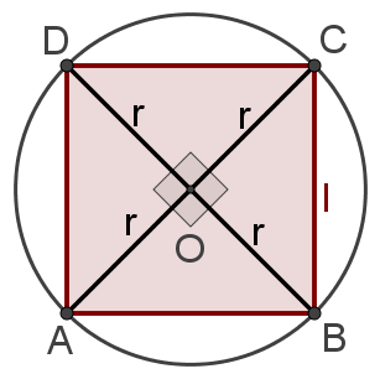
\includegraphics[width=0.36\textwidth]{ep1stern1.jpeg}
\caption{\label{fig:ep1stern1} Quadrado de raio 1 é menor que o círculo de raio 1, pois está contido nele. }
\end{figure}

\subsection{Calculando n}
Pela fórmula (1), e os valores de 2.2.3, temos:
\begin{equation}
    n = \frac{z_\gamma^2 \sigma^2}{\varepsilon^2} \implies
    n = \frac{1,96^2 \times 0,25}{0,00025} = 15366400
\end{equation}

\section{Simulando $\pi$ com pyhton}

Usamos o pacote numpy para gerar números aleatórios, visto que ele é mais eficiente que o random. usamos \textbf{np.random.uniform(0,1,n)} para gerar dois vetores, x e y, de comprimento n, em que cada valor é um número aleatório entre 0 e 1, de U(0,1). Observação: usei U(0,1) e não U(-1,1) pois não altera a proporção, e evitava contas desnecessárias para o algorítmo, que teria que fazer U(0,1)*2-1.

Após isso, tomamos cada par (x[i],y[i]) e calculamos se a distância deles para (0,0) era menor ou igual a 1, e se sim, adicionamos 1 à nossa contagem. Toda essa etapa foi feita pela linha $\textbf{cont = np.sum(x**2 + y**2}<\textbf{= 1)}$. Observação: usei $x^2 + y^2$ quando o certo seria $\sqrt{x^2 + y^2}$ pois a raíz só é menor que 1 se o número também for, e isso pouparia o computador de gastar tempo calculando essas raízes em vão.

Por fim, temos que nosso estimador $\widehat{p}$ dado pela proporção de cont/n, ou cont/15366400, ou seja, nosso $\pi$ estimado é igual a 
\[
\widehat{\pi} = 4\widehat{p} = \frac{4cont}{15366400}
\],
que é o valor retornado por \textbf{estima\_pi()}.



\section{Referências}
Bussab \& Morettin - Estatística Básica, $6^a$ edição. Editora Saraiva, 2009.


\end{document}